\documentclass[10pt,twocolumn,letterpaper]{article}

\usepackage{cvpr}
\usepackage{times}
\usepackage{epsfig}
\usepackage{graphicx}
\usepackage{amsmath}
\usepackage{amssymb}

\usepackage{subcaption}
\captionsetup{compatibility=false}

% Include other packages here, before hyperref.

% If you comment hyperref and then uncomment it, you should delete
% egpaper.aux before re-running latex.  (Or just hit 'q' on the first latex
% run, let it finish, and you should be clear).
\usepackage[pagebackref=true,breaklinks=true,letterpaper=true,colorlinks,bookmarks=false]{hyperref}

%\cvprfinalcopy % *** Uncomment this line for the final submission

\def\cvprPaperID{Occular Tension} % *** Enter the CVPR Paper ID here
\def\httilde{\mbox{\tt\raisebox{-.5ex}{\symbol{126}}}}

% Pages are numbered in submission mode, and unnumbered in camera-ready
\ifcvprfinal\pagestyle{empty}\fi
\begin{document}

%%%%%%%%% TITLE
\title{Analysis and Implementation of VSLAM Methods}

\author{Sajan Patel\\
University of Michigan\\
%Institution1 address\\
{\tt\small sajanptl@umich.edu}
% For a paper whose authors are all at the same institution,
% omit the following lines up until the closing ``}''.
% Additional authors and addresses can be added with ``\and'',
% just like the second author.
% To save space, use either the email address or home page, not both
\and
Shurjo Banerjee\\
University of Michigan\\
%Institution2\\
%First line of institution2 address\\
{\tt\small shurjo@umich.edu}
}

\maketitle
%\thispagestyle{empty}

%%%%%%%%% ABSTRACT
\begin{abstract}
The overall problem of Visual Simultaneous Localization and Mapping (VSLAM) and its different aspects have 
been researched in the computer vision community extensively. This paper critiques three papers on VSLAM 
and provides an analysis of the innovative contributions of each. Robust Large Scale Monocular Simultaneous Localization and Mapping proposes a framework for implementing VSLAM using monocular cameras. SLAM++: Simultaneous Localisation and Mapping at the Level of Objects proposes a method for VLSAM using prior knowledge of the environment and object recognition. Good Features to Track for Visual SLAM (GF-SLAM) focuses on the aspect of finding good visual features to use in VSLAM based on their temporal observability. This paper also provides an analysis of the implementation of the GF-SLAM paper and the recreation of the paper's key experiment.
\end{abstract}

%%%%%%%%% BODY TEXT
\section{Introduction}
The problem of estimating a 3D model the environment as sensed by a camera as well as estimating the 
camera's trajectory is Visual Simultaneous Localization and Mapping (VSLAM). The computer vision community has researched 
and provided innovative solutions that focus on different aspects of the overall problem. In this paper, we analyze the following three CVPR conference papers on VSLAM, discussing their innovative solution to a particular aspect of VLSAM or the problem as a whole, implementation, and subsequent conclusions: 
\begin{enumerate}
\item Robust Large Scale Monocular Visual SLAM \cite{Bourmaud_2015_CVPR}
\item SLAM++: Simultaneous Localisation and Mapping at the Level of Objects \cite{Salas-Moreno_2013_CVPR}
\item Good Features to Track for Visual SLAM \cite{Zhang_2015_CVPR} 
\end{enumerate}
We also provide an in-depth analysis of our implementation of \cite{Zhang_2015_CVPR} and the conclusions drawn from the reproduction of the paper's key experiment.

%------------------------------------------------------------------------
% Critique of Monocular VSLAM
%-------------------------------------------------------------------------
\section{Robust Large Scale Monocular Visual SLAM}
%\section{Robust Large Scale Monocular VSLAM}
\subsection{Problem Statement}
This paper focuses on the problem of using calibrated monocular cameras to perform VSLAM 
while making the 
algorithm robust, accurate, and scalable. Monocular VSLAM comes with the challenge of not being able to 
observe the scale of the scene of the environment. In order to overcome this, loop closures (returning to an observed location) need to be
 detected. This is an issue in large environments where many scenes look alike and results in an erroneous 
3D model if loop closures are not detected properly. Thus, the paper focuses not only on the general 
problem of monocular VSLAM but also tackles 
a key subproblem of dealing with loop closure.

%-------------------------------------------------------------------------
\subsection{Innovative Contribution}
To solve the problem of monocular VSLAM, the authors of \cite{Bourmaud_2015_CVPR} propose a 
framework based on three innovations:
1) a Structure from Motion (SfM) algorithm based on the \textit{Known Rotation Problem} \cite{KRot}  
is used to estimate submaps which are parts of the camera trajectory and the unknown environment,
2) a loopy belief propagation algorithm is used to efficiently aligns many submaps based 
on a graph of relative 3D similarities to produce a global map that is consistent up to a scale factor, and
3) an outlier removal algorithm that detects and removes outliers in the relative 3D similarity 
graph is used to reject wrong loop closures.

\subsection{Proposed Method}
The paper proposes a four-part framework to implement the solution monocular VSLAM: 
1) keyframe selection, 2) submap reconstruction, 3) pairwise similarity estimation, and 4) large scale 
relative similarity averaging.

\textbf{Keyframe selection:} For each frame in the captured video, Harris Points of Interest 
(PoI) are detected and tracked using a Lucas-Kanade tracker. When the Euclidean distance between 
the PoI of the current frame and previously selected keyframe is greater than a specified threshold, the 
frame is selected as a keyframe.

\textbf{Submap reconstruction:} Consecutive keyframes are clustered, and using the 
\textit{Known Rotation Problem}, a SfM algorithm is applied to each one after extracting the SURF 
PoI \cite{Surf} from all member keyframes. Loops are closed inside of each submap by 
matching these PoI between pairs of keyframes. The epipolar geometry is then calculated 
using the 5-point algorithm with RANSAC and bundle adjustment \cite{5pt, Ransac} between consecutive pairs of images 
using the SURF matches and tracked Harris PoI. The local 3D orientations are then extracted and used to 
estimate the global 3D orientation. With this, known tracks of PoI are built and 
a linear program is used to solve the \textit{Known Rotation Problem}. 
This is used to estimate the camera pose at each 
keyframe and the associated 3D point to reconstruct the submap.

\textbf{Pairwise Similarity Estimation:} Loop closures in the reconstructed submaps are 
detected by first applying a bag of words approach on the SURF descriptors of the 3D 
points in all submaps to give each submap a unique descriptor. Then, the relative 
3D similarities between each keyframe and its 10 nearest neighbors are estimated by 
matching SURF descriptors with the 3D points of each submap using a k-d tree followed by the
 3-point algorithm \cite{17} with RANSAC and nonlinear refinement on 
those matches.

\textbf{Large Scale Similarity Averaging:} To align submaps by 
estimating thier global 3D similarity to the global reference frame, a cost function on relative 
similarities is minimized by transforming the problem into a graph inference problem. 
Outliers in the graphs (representing wrong loop closures) are rejected by the 
\textit{outlier removal algorithm} \cite{Bourmaud_2015_CVPR} in which loop closures are incrementally checked 
by finding the shortest loop of inliers and adding them to an overall graph of inliers 
if their cycle error and covariance are within specified bounds. 
Once the outliers are removed, the \textit{loopy belief propagation algorithm} 
\cite{Bourmaud_2015_CVPR} performs 
graph inference by accumulating the measurements and variances on temporal 
subgraphs of the original graph as it builds up final average global similarity. 
This algorithm is parallelized, so it can be applied on a large scale of submaps.

\subsection{Experimental Evaluation}
To evaluate the proposed VSLAM framework, the authors compared its performance 
with that of state of the art algorithms in \cite{10} and \cite{12} on the TUM RGB-D \cite{29} 
and KITTI \cite{mv31} datasets and 
with four different cameras with different resolutions on indoor videos they captured. 
Each experiment used the same optimized parameters for the various parts of the algorithm. 
When evaluating the results of the algorithms with respect to ground truth, a 3D similarity 
obtained from the minimum distance between the estimated and actual camera trajectories 
was used. When compared to the \cite{10} on the TUM RGB-D dataset , the author's approach 
resulted in a 
lower RMSE for camera trajectories. 
When compared to \cite{12} on the KITTI dataset, 
the author's algorithm estimated camera trajectories that were closer to the ground truth and 
thus performed better. When compared to \cite{10} on their own videos, the proposed 
method outperformed it with respect to the ground truth motion of the camera. 
In addition, the paper discusses the limitations of the framework in not being able to 
estimate a pure rotation of the camera, the necessity for the sensed environment 
to be static, and the necessary for consecutive relative similarities to be outlier free. 
However, the framework still has reasonable performance when applied to datasets 
that involve some moving objects.

\subsection{Subsequent Conclusions}
The performance evaluation of the method shows that the authors' proposed monocular VSLAM framework does
 substantiate their claim. Robust, independent submap generation is achieved by the visual odometry approach 
based on the \textit{Known Rotation Problem}, and these submaps can be processed and aligned to form the 
global map and camera trajectory estimates with loop closure through the outlier removal and loopy belief 
propagation algorithms. Even with the described limitations, the evaluations show the innovative framework does 
provide a robust, accurate, and scalable solution to loop closure and the overall problem monocular VSLAM.

\section {SLAM++: Simultaneous Localisation and Mapping at the Level of Objects}
%\section{SLAM++}
\subsection{Problem Statement}
This paper focuses on the problem of implementing VSLAM at the level of 3D objects rather than low-level 
primitives (i.e. points, lines, etc) that must be robustly matched. Moreover, much of the prior knowledge of
 objects and the environment could be taken into account ``in the loop" of the VSLAM algorithm itself but is 
 currently wasted \cite{Salas-Moreno_2013_CVPR}. Thus, the authors of \cite{Salas-Moreno_2013_CVPR} 
 aim to solve the problem of implementing VSLAM with higher level features that can take into account the semantic labelling of geometry as objects and regions provided by the improved, efficient, and powerful hardware that exists today.

%-------------------------------------------------------------------------
\subsection{Innovative Contribution}
To solve the problem of VSLAM approached from the perspective of 3D object recognition, the authors of \cite{Salas-Moreno_2013_CVPR} propose the innovation of building pose graph maps based on an ``object-oriented" approach that directly encodes the positions of recognized 3D structures. With each new sensor measurement, the graph is continually optimized and allows for efficient tracking of the camera system based on recognized landmarks. In addition to this, the algorithms make the assumption that the world has ``intrinsic symmetry in the form of repetitive objects" \cite{Salas-Moreno_2013_CVPR} thereby allowing for the the objects in a scene to be identified and segmented as salient repeated elements. KinnectFusion algorithms are used to scan and detect objects matched to previously created models which are then used in camera pose tracking. The algorithm leverages this repetitiveness along with the efficient use of GPU architectures to provide a real time processing system. 

%-------------------------------------------------------------------------
\subsection{Proposed Method}
\textbf{Creating an Object Database:} First, a database of models repeatedly occurring objects is created via known KinectFusion algorithms \cite{kf11}. 
These are objects that are subsequently recognized and used in the VSLAM process. 

\textbf{SLAM Map Representation:} The world is represented by a graph where each node stores the 6DOF 
pose of discovered objects relative to a fixed world frame as well as an annotation of the label of the object from the database that it matches to.

\textbf{Real-Time Object Recognition:} This portion of the method recognizes objects in the world based on standard mesh recognition algorithms similar to those in \cite{drost6}. The implementation is parallelized on GPUs to allow the real-time detection of multiple instances of multiple objects. These correspondences are obtained via the use of Point-Pair Features (PPFs) which are 4D descriptors of relative poses and pairs of oriented surface normals for each object. 

\textbf{Camera Tracking and Object Pose Estimation:} The iterative closest point (ICP) algorithm \cite{icp15} is used to to track the pose of the camera model based on the earlier computed object based locations. A Huber penalty function is used to in this optimization process. Criteria is developed to ensure successful convergence of the tracking error.

\textbf{Graph Optimization:} The poses of each static object are now viewed as a graph optimization problem which minimizes the sum over all the measurement constraints based on the known features of each object.

\textbf{Relocalization:} The system accounts for a loss in camera tracking by reinitializing localization based on matching at least three of the objects seen in the previously tracked long-term graph. 

%-------------------------------------------------------------------------
\subsection{Experimental Evaluation}
The authors of \cite{Salas-Moreno_2013_CVPR} reference a video submitted along with it to CVPR as a better description of the advantages of their method. 

\textbf{Loop Closure:} Small loop closures are detected and compensated for by the ICP algorithm. Larger loop closures are compensated for by the relocalization method. 

\textbf{Large Scale Mapping:} Scaled mapping of a large room (15mX10mX3m) was obtained along with the mapping of 34 different objects around the room. The algorithm uses no priors regarding the original placement of these objects.

\textbf{Moved Object Detection:} The algorithm also displays the ability to track these objects while they, themselves are in motion. 

\textbf{System Statistics:} The algorithm displays the amount of storage used as compared to the more traditional KinectFusion algorithm. The given mapped rooms is stored in about 20MB of space as compared to the 1.4GB used by KinectFusion. The resultant compression ratio is 1/70 which is a dramatic improvement. 

%-------------------------------------------------------------------------
\subsection{Subsequent Conclusions}
The authors of \cite{Salas-Moreno_2013_CVPR} makes several bold claims with regard to its own contributions to the literature. The graph based optimization method does indeed seem novel and the system has significantly large data compression ratio when compared to the KinectFusion algorithms. Unfortunately, the experimentally evaluated conclusions are quite sparse when compared to the dense and well-written introduction and methodology of the paper. The biggest issue pertains to the fact that no standard metric is used to compare the system's advantages and efficiently to other 3D-object-recognition-based VSLAM approaches. Though several claims are made about the paper's VSLAM advantages over other methods, there are no easy ways to determine the validity of these claims.

%%%%%%%%%%%%%%%%%%%%
\section {Good Features to Track for VSLAM}
\subsection{Problem Statement}
This paper focuses on the problem of feature selection for VSLAM since not all features 
detected and tracked by conventional methods contribute to the accurate estimation of 
camera trajectories and the overall map. Only a subset of all tracked and detected features 
actually produces a good result for VSLAM, and furthermore, there are many different ways of
detecting these features. As VSLAM applications grow to include large-scale reconstruction from
 large sets of features, an efficient algorithm that can be applied to features generated by any 
detection method is necessary. Thus, this paper focuses on finding the best features out of any given 
set of previously detected features as a preprocessing step for VSLAM.

In exploring different methods for VSLAM proposed in recent conference papers, 
we chose to re-implement the methods and key experiment of this paper.

\subsection{Innovative Contribution}
To solve the problem of finding the best features to use for VSLAM given a set of detected features, 
\cite{Zhang_2015_CVPR} proposes a new SVD-based algorithm for more rigorous feature selection to be used 
during the localization process. The paper develops a mechanism by which such measured features 
can be ranked with an observability score. The ranked feature set can then be used to generate a 
reduced feature set with better a better estimation accuracy. The authors call their system the \textit{Good 
Features} algorithm (GF-SLAM for short). The innovative contribution of this paper is in the three main 
aspects of GF-SLAM: 1) a system observability measure for features, 2) a rank-k temporal update 
of observability scores, and 3) a submodular learning method for completing the set of good features if 
the initial ranking of scores fails to provide the desired quantity of good features for a given application of 
VSLAM.

\textbf{System Observability Measure}: To counter the use of extraneous features in the localization process 
of VSLAM, the paper develops a metric of observability scores based on the temporal observability 
for each detected feature in each captured video frame. Features are represented by their coordinates in the 
image plane as well as the corresponding world coordinates, allowing this measure to be applied to features 
extracted from video frames by any detection method. The general idea is that features with higher temporal 
observability are scored higher and the set of \textit{good features} is created from all features whose scores are 
above a specified threshold based on the application of VSLAM. These good features are then called 
anchors.

\textbf{Rank-k Temporal Update of Observability Score}: The generation of feature observability 
scores requires 
the computation and storage of large observability matrices that increase over time. 
The actual act of creating these matrices is inefficient and can lead to delays 
in the SLAM process. To counter this, the authors propose a new algorithm to generate the 
observability matrix 
based on an incremental SVD of the system's observability matrix applied per time step.

\textbf{Submodular Learning for Feature Grouping}: The ranking and thresholding of feature 
observability scores may not 
always produce an adequate number of anchors. 
Thus, this paper proposes a submodular learning algorithm that 
greedily chooses the best of the remaining features with scores 
below the threshold to complete the anchor set based on an 
SVD of the augmented system observability matrix of the anchor set and possible upgraded features. 

\subsection{Proposed Method}
\textbf{Dynamical Measurement Model of VSLAM System:}
The authors use a constant velocity motion model that describes the motion of a VSLAM system in standard 
Euclidian three space, 
$SE(3)$, as the basis for their algorithm. The method requires the position and orientation as well as the linear 
and angular velocities of the camera model of the VSLAM system: 
\begin{equation} \label{eq:stateVector}
\boldsymbol{x}_{R_k}^W = (\boldsymbol{r}_{R_k}^W \ \ \ \  \boldsymbol{q}_{R_k}^W  \ \ \ \  \boldsymbol{v}_{R_k}^W  \ \ \ \  \boldsymbol{\omega}_{R_k}^W)^T
\end{equation}
where $\boldsymbol{x}_{R_k}^W$ is the state vector of the camera model, 
$\boldsymbol{r}_{R_k}^W$ is its position, 
$\boldsymbol{v}_{R_k}^W$ is its velocity, 
and $\boldsymbol{\omega}_{R_k}^W$ is its angular velocity. All these quantities are with reference to the world frame as denoted by the superscript $W$ at time $k$. 
The state vector is updated with each time segment by the SLAM system. 

The algorithm requires access to the following properties of the features that are located by the SLAM system: 
\begin{equation} \label{eq:featureProjection}
\boldsymbol{p}_{i}^{R_k} = ({p}_{x_i}^{R_k} \ \ \ \  {p}_{y_i}^{R_k}  \ \ \ \  {p}_{z_i}^{R_k})^T = R^{R_k}_{W}((\boldsymbol{q}^{W}_{R_k})^{-1})(^{(i)}\boldsymbol{p}^{W}_{k} - \boldsymbol{r}^{W}_{R_k})
\end{equation}
\begin{equation} \label{eq:featureProjection2}
\boldsymbol{h}_{i}^{R_k} = \begin{bmatrix} {h}_{x_i} \\ {h}_{y_i} \end{bmatrix} = distort(\begin{bmatrix}
u_0 - fk_u\frac{p_x^{R_k}}{p_z^{R_k}}\\
v_0 - fk_u\frac{p_y^{R_k}}{p_z^{R_k}}
\end{bmatrix})
\end{equation}
where $\boldsymbol{p}_{i}^{R_k}$ is the pinhole projection of the features,  
$\boldsymbol{h}_{x_i}$ is the projection of these coordinates on to the 2D pinhole plane, $R(\boldsymbol{q})$ is the rotation matrix of $\boldsymbol{q}$, and $fk_u, fk_v, u_0, and v_0$ are the camera's intrinsic parameters.
These coordinates are obtained after correcting for distortion which involves the intrinsic parameters of the camera via the $distort(.)$ function from \cite{distort}.

\textbf{Computation of System Observability Measure:} To compute the observability score for each feature,
\cite{Zhang_2015_CVPR} defines a System Observability Matrix (SOM), ${Q}_{SOM}$ based on \cite{gf15}. ${Q}_{SOM}$ is defined for a fixed number 
of frames, $\tau$, of the SLAM process. When the current frame iteration grows larger than $\tau$, the oldest
 elements of the now fixed size ${Q}_{SOM}$ are replaced directly by the newest feature values. $\tau$ is 
 thus an important input parameter to the system as it governs the efficiency of the overall algorithm. 
 ${Q}_{SOM}$ itself is built as a function of the current frame number, $j$, where 
 $j<\tau$. 
\begin{equation} \label{eq:qsom}
\boldsymbol{Q}_{SOM}(j) = \begin{bmatrix} \ \ Q_1^T \ | \ Q_2^T \ | \ ... \ | \ Q_j^T  \ \ \end{bmatrix}
\end{equation}

The replacement process for when $j>\tau$ is described in a later section. Each $Q_j^T$ is built and appended to ${Q}_{SOM}$ as the frame number increments. Each $Q_j^T$ itself has the following form: 
\begin{equation} \label{eq:Qjjj}
Q_j^T = \begin{bmatrix} \ \ H_j^T \ | \ (H_j F_j)^T \ | \ ... \ | \ (H_j F_j^{n-1})^T  \ \ \end{bmatrix}
\end{equation}
where $F$ is the process matrix that relates the motion model defined in \eqref{eq:stateVector} 
from one state to the next. $H$ is the measurement Jacobian where the derivatives are arranged as follows (with features and anchors abbreviated as ``feat." and ``anch." respectively):
\\\\
$\begin{bmatrix}
\small{\text{image feat. w.r.t. camera state}}&\small{\text{image feat. w.r.t. world feat.}}\\
\small{\text{image anch. w.r.t. camera state}}&0
\end{bmatrix}$\\

Once $Q_{SOM}$ is computed, the temporal observability scores for each feature is computed as:
\begin{equation} \label{eq:Qjjj}
score(f) = \sigma_{min}(Q_{SOM} \ for \ feature \ f)
\end{equation}

\textbf{Rank-k Temporal Update of Observability Score:} As can be seen from the preceding section, the computation of $Q_{SOM}$ is an extensive operation. To simplify matters the authors present an iterated SVD approach to creating $Q_{SOM}$ when $j>3$  and $j<\tau + 1$. 

Fundamentally, $Q_{SOM}$ is created via \eqref{eq:qsom} 
for the first three frames. For subsequent frames, the SVD of $Q_{SOM}$ is combined with the corresponding calculated ${Q}_{j}$ in \eqref{eq:Qjjj} to form the new $Q_{SOM}$. Again, this new definition of several matrices and involves the diagonalization of newly constructed matrices. 

\textbf{FIX THIS AND ADD THE RANK-K UPDATE HERE!!!! We can't ask readers to read the GF Paper since we're supposed to be explaining it to them.}
Please refer to the original text for the complete implementation details. The net gain by the algorithm is the creation of $Q_{SOM}$ by a rank-2r update instead of creating a whole new matrix. 

For $j>\tau + 1$ , $Q_{SOM}$ is updated via replacement. The newest ${Q}_{j}$ in \eqref{eq:Qjjj} is computed and placed in the positions occupied by the oldest elements of the matrix. As an example, if at time k, $Q_{SOM}(k) = \begin{bmatrix} \ \ Q_1^T \ | \ Q_2^T \ | \ ... \ | \ Q_k^T  \ \ \end{bmatrix}$, then at time k+1, the oldest (i.e. the first element) is replaced, ${Q}_{SOM}(k+1) = \begin{bmatrix}\ \ Q_{k+1}^T \ | \ Q_2^T \ | \ ... \ | \ Q_k^T\ \ \end{bmatrix}$.

\textbf{Submodular Learning for Feature Grouping:} If the set of anchors created after the thresholding of the feature observability scores is smaller than desired, a greedy submodular learning algorithm upgrades features with with the next best scores to anchors to complete the anchor set. This is done by creating an SOM of just the anchors and candidate rows for each remaining feature. The algorithm iterates through each candidate feature, appending it's row to the end of the anchor SOM and then taking the SVD of that matrix to get the observability score for that feature via \eqref{eq:Qjjj} with the modification that $Q_{SOM}$ is now the anchor and candidate row SOM. The feature whose row produces the maximum observability score is upgraded to be an anchor and removed from the set of features. This greedy algorithm recomputes the anchor and candidate SOMs and repeats the process until the the desired number of anchors is obtained.

\subsection{Experimental Method}
The feature reduction algorithm was implemented on readily 
available simulated VSLAM data that was created for \cite{31}. 
The robot is made to move in a circle in a simulated environment of dimensions 12mX12m with 72 
landmarks forming a square. The VSLAM process uses an Extended Kalman Filter (EKF) to estimate the locations 
of each landmark and subsequent estimate its own position in the map. In the original EKF algorithm, the 
simulated robot detects as many landmarks that it can detect. The authors apply their SVD ranking approach
 to select a certain subset of the number of features selected. By changing the number of features used as 
 well as the observation noise, they run the VSLAM simulation several times and compare their results to 
 that of the original algorithm. They run each simulation 40 times and count the number of times their 
 algorithm outperforms the original. The noise values used are $\sigma=\{0.5, 1.0, 1.5, 2.0, 2.5\} $. 
The number of features used are $ K = \{ 3, 4, 5, 6, 7, 8, 10, 12 \}$. 
The results are provided in Table 1. 

%%%%%%%%%%%%%%%%%%%%%%
\begin{figure*}[t!]
        \begin{subfigure}[b]{0.25\textwidth}
                \fbox{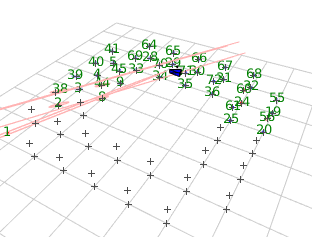
\includegraphics[height = 3.5cm, width=\linewidth]{Figures/AllFeatures_SLAM.png}}
                \caption{VSLAM (all features)}
                \label{fig:gull}
        \end{subfigure}%
        \begin{subfigure}[b]{0.25\textwidth}
                \fbox{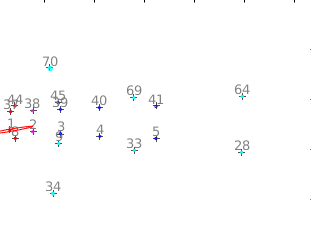
\includegraphics[height = 3.5cm, width=\linewidth]{Figures/AllFeatures_Pinhole.png}}
                \caption{Pinhole View (all features)}
                \label{fig:gull2}
        \end{subfigure}%  
        \begin{subfigure}[b]{0.25\textwidth}
                \fbox{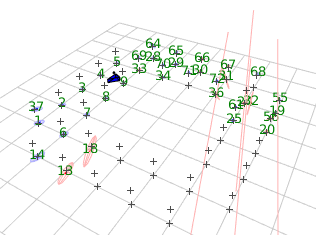
\includegraphics[height = 3.5cm, width=\linewidth]{Figures/FewerFeatures_SLAM.png}}
                \caption{VSLAM (10 ranked feat.)}
                \label{fig:tiger}
        \end{subfigure}%
        \begin{subfigure}[b]{0.25\textwidth}
                \fbox{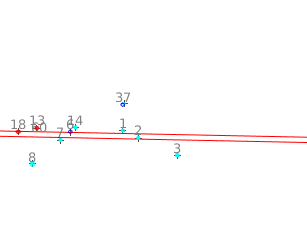
\includegraphics[height = 3.5cm, width=\linewidth]{Figures/FewerFeatures_Pinhole.png}}
                \caption{Pinhole View (10 ranked feat.)}
                \label{fig:mouse}
        \end{subfigure}
        \caption{Experimental Results: (a) VSLAM is performed using all the features. All the landmarks (+ signs) are detected by the robot and used for localization. (b) Shows the pinhole view of the robot in the first scene. These pixel coordinates form the $\boldsymbol{h}_{x_i}$ that \eqref{eq:featureProjection2} used in the algorithm. (c) VSLAM is performed with the the 10 highest ranked features. In the figure this is apparent from the fact that all the landmarks in the vicinity of the robot are not labelled. (d) Corresponding pinhole view. As expected, fewer features are being used for the localization process.}
\label{fig:animals}
\end{figure*}
%%%%%%%%%%%%%%%%%%%%%%

\subsection{Our Implementation}
We chose to re-implement the method and key experiment of \cite{Zhang_2015_CVPR}. The first step was to run the original EKF-VSLAM algorithm in \cite{31} that was used by \cite{Zhang_2015_CVPR} in its experimentation. The code for \cite{31} was readily available to download and use online.

\textbf{Algorithm Structure:} The algorithm simulates a robot moving in a circular trajectory surrounded by 72 detectable landmarks. A monocular camera is placed on the robot for visual sensing purposes. Broadly the algorithm is divided in to the following sections:
\begin{enumerate}
  \item \textit{Data Generation}: The trajectory to be followed by the robot is generated. Each landmarks's position is also generated. Care is taken to seed the random number generator at a fixed point so as to ensure consistency across measurements.
  \item \textit{Simulation}: The simulated robot is moved ahead on the predefined trajectory. The measurement vectors are generated based on the location of the landmarks located by the robot. In the terms of our implementation, we consider the features to be these landmark positions. 
 \item \textit{Localization}: The robot's current position and orientation is localized by sending all the detected features to an Extended Kalman Filtering Algorithm.
\item \textit{Visualization}: The corresponding position of the landmarks, detected features, actual robot's position and orientation and estimated robot's position and orientation are visually updated on a three dimensional plot.
\end{enumerate}

\textbf{Calculating $\boldsymbol{Q}_{SOM}$:} The first step in generating the observability matrix is mapping  features detected by the SLAM algorithm to their corresponding $\boldsymbol{p}_{i}^{R_k}$'s from \eqref{eq:featureProjection} and $\boldsymbol{h}_{x_i}$ from \eqref{eq:featureProjection2}. This is done between step 2 and 3 by extracting the corresponding elements from the algorithms pinhole perspective calculations. The camera's corresponding position and orientation, $\boldsymbol{x}_{R_k}^W$, is also extracted by  \eqref{eq:stateVector}. These features are used to create a corresponding $H$ matrix which in turn is used to iteratively build up $Q_{SOM}$ as described in \eqref{eq:qsom} and \eqref{eq:Qjjj}. $Q_{SOM}$ is created to contain information from 10 iterations of the EKF algorithm at a time i.e. $\tau = 10$. As described previously, $Q_{SOM}$ is initially created iteratively, then via the iterative SVD and finally via the replacement method.
  
\textbf{Feature Scoring:} Step two provides us with a list of features that has been detected by the robot. Each of these features have corresponding rows in the $Q_{SOM}$ matrix. For each feature, the corresponding rows are iteratively extracted and concatenated to form a feature matrix. 
The SVD is computed for each of these matrices and the minimum positive singular value is extracted as a
 corresponding score of each feature by \eqref{eq:qsom}. 
 The resultant scores are then used to sort the original features as well 
as the corresponding $\boldsymbol{p}_{i}^{R_k}$'s and $\boldsymbol{h}_{x_i}$'s. A subset of the scored features with scores above an 
application-specified threshold is designated as the anchor set and is passed on to the localization step and the algorithm proceeds as normal.\\
\indent{}\textbf{Submodular Learning:} We implemented submodular learning to complete the anchor set as described by the paper's proposed greedy algorithm. This portion of the implementation also runs only if the resultant set of anchors after thresholding the feature scores is less than two below the desired number of 
anchors.\\
\indent{}\textbf{Experimental Implementation:} The experiment described in \cite{Zhang_2015_CVPR} was recreated exactly.
\textbf{(WTF is this saying? Did we run 40 times 200 iterations?) A total of 40 experiments were performed at a fixed seeded location.} The experiment sweeps over 200 iterations for each combination of pixel noise and number of anchors from the follow sets: $\sigma=\{0.5, 1.0, 1.5, 2.0, 2.5\} $ and $ K = \{ 3, 4, 5, 6, 7, 8, 10, 12 \}$. The positional and Euclidian L2-norms are used to compare the results of the original algorithm and our.\\
\indent{}\textbf{Experimental Results:} Figure 1 shows the results of the experiment. Table 2 results obtained in terms of the positional norm. 
Table 3 provides the results obtained in terms of the Euclidian norm. 
Our implementation performed better then the original in 8/40 cases (20\%) in terms of the positional norm. 
In terms of the Euclidian norm, it performed better in 14/40 cases (35\%).
%----
\begin{table}[h]
\begin{center}
\begin{tabular}{|c|c|c|}
\hline
Metric Used & Num. Successful & Accuracy  \\
\hline
 Translation Error &   &   \\
$ \sum_k || \Delta \boldsymbol{r}_{R_k}^W ||_2 $ & 37/40 & 92.5\% \\ 
%&   &   \\
\hline
Rotation Error &   &   \\
$ \sum_k || \Delta \boldsymbol{\theta}_{R_k}^W ||_2 $ & 33/40 & 82.5\% \\
%&   & \\
\hline
\end{tabular}
\end{center}
\caption{Author's experimental results.}
\end{table}
%-0-----------
\begin{table}[h]
\begin{center}
\begin{tabular}{|c|c|c|}
\hline
$\sigma$ & Avg. ($ \sum_k || \Delta \boldsymbol{r}_{R_k}^W ||_2)_{all} $ & Avg. ($ \sum_k || \Delta \boldsymbol{r}_{R_k}^W ||_2)_{rnk} $ \\
\hline
0.5  & 6.3591  &  7.0524\\
\hline
1.0  &  4.8382 &  8.9654\\
\hline
1.5  &  6.1305 &  10.1870\\
\hline
2.0  &  6.5744 &  7.0839\\
\hline
2.5  &  6.4082 &  8.5952\\
\hline
\end{tabular}
\end{center}
\caption{Position Based Results}
\end{table}
\begin{table}[t]
\begin{center}
\begin{tabular}{|c|c|c|}
\hline
$\sigma$ & Avg. ($\sum_k || \Delta \boldsymbol{\theta}_{R_k}^W ||_2)_{all}$ & Avg. ($ \sum_k || \Delta \boldsymbol{\theta}_{R_k}^W ||_2)_{rnk}$\\
\hline
0.5  & 0.7082  &  7.2744\\
\hline
1.0  &  0.9237 &  5.8175\\
\hline
1.5  &  0.8389 &  8.5750\\
\hline
2.0  &  7.9474 &  4.7680\\
\hline
2.5  &  8.0217 &  6.1176\\
\hline
\end{tabular}
\end{center}
\caption{Euclidian Norm Based Results}
\end{table}
%--------------

\subsection{Subsequent Conclusions}
As can be seen, the results we obtained do not agree with those in \cite{Zhang_2015_CVPR} though the experiment (including all procedures, parameters, and metrics) was reproduced exactly. We believe the reason for this an incorrect creation of the $Q_{SOM}$ matrix. This paper turned out to be particularly difficult to re-implement. The main reason behind this was the convoluted mathematical definitions and notations used by the authors especially with regard to the contents and creation of $Q_{SOM}$, including each feature's temporal contribution of a row to the matrix and the correspondence of the matrix's singular values to individual features. We tried to contact the authors via email but are unfortunately yet to hear back from them. They also do not provide any of the software or code used.

Based on the metrics they define, the author's feature scoring algorithm appears to successfully aid VSLAM processes. Unfortunately, their results do not appear to be easy to reproduce. For this algorithm to achieve more success in the community it is our suggestion that the authors clean up their mathematical notation as well as release commented software and code which performs the algorithm successfully.    

\section{Conclusion}
The vision community has done much research in the area of VSLAM and its various aspects. Through this paper, we present an analysis of three papers' innovative methods: large-scale monocular VSLAM that is robust to observed data size in \cite{Bourmaud_2015_CVPR}, KinnectFusion-based VSLAM that relies on 3D object recognition and prior models of those objects in \cite{Salas-Moreno_2013_CVPR}, and the selection of a subset of detected features to use for VSLAM based on their temporal observability in \cite{Zhang_2015_CVPR}. We also present our implementation of GF-SLAM from \cite{Zhang_2015_CVPR} and the results and conclusions drawn from our attempt to recreate the main experiment it was originally tested on. 

{\small
\bibliographystyle{ieee}
\bibliography{sajanptl_shurjo}
}

\end{document}
